\documentclass{beamer}
\mode<presentation>
\usepackage{amsmath,amssymb,mathtools}
\usepackage{textcomp}
\usepackage{listings}
\usepackage{adjustbox}
\usepackage{gensymb}
\usepackage{url}
\usepackage{subcaption}
\usepackage{graphicx}
\def\UrlBreaks{\do\/\do-}
\usetheme{Boadilla}
\usecolortheme{lily}
\setbeamertemplate{footline}{
  \leavevmode%
  \hbox{%
  \begin{beamercolorbox}[wd=\paperwidth,ht=2ex,dp=1ex,right]{author in head/foot}%
    \insertframenumber{} / \inserttotalframenumber\hspace*{2ex}
  \end{beamercolorbox}}%
  \vskip0pt%
}
\setbeamertemplate{navigation symbols}{}
\lstset{
  frame=single,
  breaklines=true,
  columns=fullflexible,
  basicstyle=\ttfamily\tiny
}
\numberwithin{equation}{section}
\providecommand{\nCr}[2]{\,^{#1}C_{#2}}
\providecommand{\nPr}[2]{\,^{#1}P_{#2}}
\providecommand{\mbf}{\mathbf}
\providecommand{\pr}[1]{\ensuremath{\Pr\left(#1\right)}}
\providecommand{\qfunc}[1]{\ensuremath{Q\left(#1\right)}}
\providecommand{\sbrak}[1]{\ensuremath{{}\left[#1\right]}}
\providecommand{\lsbrak}[1]{\ensuremath{{}\left[#1\right.}}
\providecommand{\rsbrak}[1]{\ensuremath{\left.#1\right]}}
\providecommand{\brak}[1]{\ensuremath{\left(#1\right)}}
\providecommand{\lbrak}[1]{\ensuremath{\left(#1\right.}}
\providecommand{\rbrak}[1]{\ensuremath{\left.#1\right)}}
\providecommand{\cbrak}[1]{\ensuremath{\left\{#1\right\}}}
\providecommand{\lcbrak}[1]{\ensuremath{\left\{#1\right.}}
\providecommand{\rcbrak}[1]{\ensuremath{\left.#1\right\}}}
\theoremstyle{remark}
\newtheorem{rem}{Remark}
\newcommand{\sgn}{\mathop{\mathrm{sgn}}}
\providecommand{\abs}[1]{\left\vert#1\right\vert}
\providecommand{\res}[1]{\Res\displaylimits_{#1}}
\providecommand{\norm}[1]{\lVert#1\rVert}
\providecommand{\mtx}[1]{\mathbf{#1}}
\providecommand{\mean}[1]{E\left[ #1 \right]}
\providecommand{\fourier}{\overset{\mathcal{F}}{ \rightleftharpoons}}
\providecommand{\system}{\overset{\mathcal{H}}{ \longleftharpoons}}
\providecommand{\dec}[2]{\ensuremath{\overset{#1}{\underset{#2}{\gtrless}}}}
\newcommand{\myvec}[1]{\ensuremath{\begin{pmatrix}#1\end{pmatrix}}}
\newcommand{\mydet}[1]{\ensuremath{\begin{vmatrix}#1\end{vmatrix}}}
\let\vec\mathbf
 
\title{Analog -- Problem 1.1.56}
\author{ee25btech11056 -- Suraj.N}
 
\begin{document}
 
%-------------------------------------------------------------
\begin{frame}
  \titlepage
\end{frame}
 
%-------------------------------------------------------------
\begin{frame}{Problem Statement}
 
\textbf{Problem 1.1.56} 

Consider the triangular wave generator shown in Fig.\,1.1.56.1.
Assume ideal op-amps with $\pm2\,\mathrm{V}$ supply.
The input is a $+5\,\mathrm{V}$, 50\,Hz square wave with 50\% duty cycle.

The condition that results in a triangular wave of 5\,V peak-to-peak
and 50\,Hz at the output is:

\begin{enumerate}
  \item $RC = 1$
  \item $R/C = 1$
  \item $R/C = 5$
  \item $C/R = 5$
\end{enumerate}

\end{frame}

%-------------------------------------------------------------
\begin{frame}{Circuit Diagram}

\begin{figure}[h!]
  \centering
  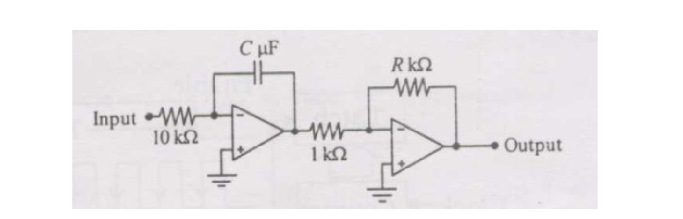
\includegraphics[width=1\columnwidth]{figs/circuit.png} 
  \caption*{Fig : Circuit}
  \label{Fig1}
\end{figure}



\end{frame}

\begin{frame}{Step 1: Deriving Output of Integrator Circuit}
 
For an ideal op-amp with negative feedback:
 
\begin{enumerate}
  \item The open-loop gain $A \to \infty$
  \item The differential input voltage $V^+ - V^- \to 0$
  \item Since $V^+ = 0$ (grounded), we get $V^- = 0$
\end{enumerate}
 
The inverting terminal is therefore at \textbf{virtual ground}:
\[
  V^- = V^+ = 0\,\mathrm{V}
\]
 
This means the voltage across $R_1$ is simply $V_{\mathrm{in}} - 0 = V_{\mathrm{in}}$.
 
The current through $R_1$ flowing into the virtual ground node is:
\[
  i_{R_1}(t) = \frac{V_{\mathrm{in}}(t) - V^-}{R_1} = \frac{V_{\mathrm{in}}(t)}{R_1}
\]
 
\end{frame}
 
%-------------------------------------------------------------
\begin{frame}{Step 2: KCL at the Inverting Terminal}
 
Since the ideal op-amp draws \textbf{zero input current}, all of
$i_{R_1}$ must flow through the capacitor $C$.
 
Applying KCL at the inverting node $V^-$:
\[
  i_C(t) = \frac{V_{\mathrm{in}}(t)}{R_1}
\]
 
The voltage--current relationship for the capacitor is:
\[
  i_C(t) = C\,\frac{d}{dt}\bigl(V^- - V_{\mathrm{out}}(t)\bigr)
           = C\,\frac{d}{dt}\bigl(0 - V_{\mathrm{out}}(t)\bigr)
           = -C\,\frac{dV_{\mathrm{out}}(t)}{dt}
\]
 
\end{frame}
 
%-------------------------------------------------------------
\begin{frame}{Step 3: Differential Equation}
 
Equating the two expressions for $i_C(t)$:
\[
  -C\,\frac{dV_{\mathrm{out}}(t)}{dt} = \frac{V_{\mathrm{in}}(t)}{R_1}
\]
 
Rearranging:
\[
  \frac{dV_{\mathrm{out}}(t)}{dt} = -\frac{V_{\mathrm{in}}(t)}{R_1 C}
\]
 
This is the governing differential equation of the inverting integrator.
The output voltage changes at a rate proportional to the input voltage,
with a sign inversion and scaling by $\dfrac{1}{R_1 C}$.
 
\end{frame}
 
%-------------------------------------------------------------
\begin{frame}{Step 4: Integration to Get Output Formula}
 
Integrating both sides of the differential equation from $0$ to $t$:
\[
  \int_0^t \frac{dV_{\mathrm{out}}(\tau)}{d\tau}\,d\tau
  = -\frac{1}{R_1 C}\int_0^t V_{\mathrm{in}}(\tau)\,d\tau
\]
 
The left side evaluates directly:
\[
  V_{\mathrm{out}}(t) - V_{\mathrm{out}}(0)
  = -\frac{1}{R_1 C}\int_0^t V_{\mathrm{in}}(\tau)\,d\tau
\]
 
Assuming the capacitor is initially uncharged, $V_{\mathrm{out}}(0) = 0$:
\[
  \boxed{V_{\mathrm{out}}(t) = -\frac{1}{R_1 C}\int_0^t V_{\mathrm{in}}(\tau)\,d\tau}
\]
 
This is the \textbf{inverting integrator output formula}.
 
\end{frame}


%-------------------------------------------------------------
\begin{frame}{Circuit Description}

The circuit has two stages:

\begin{enumerate}
  \item \textbf{Stage 1 -- Inverting Integrator}: input resistor
        $R_1 = 10\,\mathrm{k}\Omega$, feedback capacitor $C\,\mu\mathrm{F}$.
        Converts the square wave to a triangular ramp.
  \item \textbf{Stage 2 -- Inverting Amplifier}: input resistor
        $1\,\mathrm{k}\Omega$, feedback resistor $R\,\mathrm{k}\Omega$.
        Inverts and scales the triangular ramp.
\end{enumerate}

The transfer functions are:
\[
  V_{\mathrm{int}}(t) = -\frac{1}{R_1 C}\int_0^t V_{\mathrm{in}}(\tau)\,d\tau
\]
\[
  V_{\mathrm{out}} = -\frac{R\,[\mathrm{k}\Omega]}{1\,[\mathrm{k}\Omega]}\,V_{\mathrm{int}}
  = -R\;V_{\mathrm{int}}
\]

\end{frame}

%-------------------------------------------------------------
\begin{frame}{Input Signal}

The input is a bipolar square wave of amplitude $V_p = 5\,\mathrm{V}$:
\[
  V_{\mathrm{in}}(t) =
  \begin{cases}
    +5\,\mathrm{V} & 0 \le t  < T/2 \\
    -5\,\mathrm{V} & T/2 \le t < T
  \end{cases}
\]

The time parameters are:

\begin{enumerate}
  \item Frequency: $f = 50\,\mathrm{Hz}$
  \item Period: $T = 1/f = 20\,\mathrm{ms}$
  \item Half-period: $T/2 = 10\,\mathrm{ms} = 0.01\,\mathrm{s}$
  \item Amplitude: $V_p = 5\,\mathrm{V}$
\end{enumerate}

A bipolar square wave integrated over each half-period produces a
linear ramp. Alternating positive and negative half-cycles produce
a triangular wave at Stage 1 output.

\end{frame}

%-------------------------------------------------------------
\begin{frame}{Stage 1: Integrator Analysis}

The ramp magnitude over one half-period is:
\[
  \Delta V_{\mathrm{int}}
  = \frac{V_p \cdot (T/2)}{R_1 \cdot C}
\]

Substituting $V_p = 5\,\mathrm{V}$, $T/2 = 0.01\,\mathrm{s}$,
$R_1 = 10^4\,\Omega$, $C_{1} = C \times 10^{-6}\,\mathrm{F}$:
\[
  \Delta V_{\mathrm{int}}
  = \frac{5 \times 0.01}{10^4 \times C \times 10^{-6}}
  = \frac{0.05}{0.01\,C}
  = \frac{5}{C}\;\mathrm{V}
\]

Since the $-5\,\mathrm{V}$ half-cycle produces an equal upward ramp,
the peak-to-peak at Stage 1 output is:
\[
  \Delta V_{\mathrm{int,pp}} = \frac{5}{C}\;\mathrm{V}
  \]

\end{frame}

%-------------------------------------------------------------
\begin{frame}{Stage 2: Amplifier }

Stage 2 gain magnitude:
\[
  \left|A_v\right| = \frac{R\,[\mathrm{k}\Omega]}{1\,[\mathrm{k}\Omega]} = R
\]

Peak-to-peak at Stage 2 output:
\[
  V_{\mathrm{out,pp}} = R \times \frac{5}{C} = \frac{5R}{C}
\]

Setting $V_{\mathrm{out,pp}} = 5\,\mathrm{V}$:
\[
  \frac{5R}{C} = 5
  \quad\Longrightarrow\quad
  \frac{R}{C} = 1
  \]

\end{frame}

%-------------------------------------------------------------

\begin{frame}{Plot of Waveforms} 

\begin{figure}[h!]
  \centering
  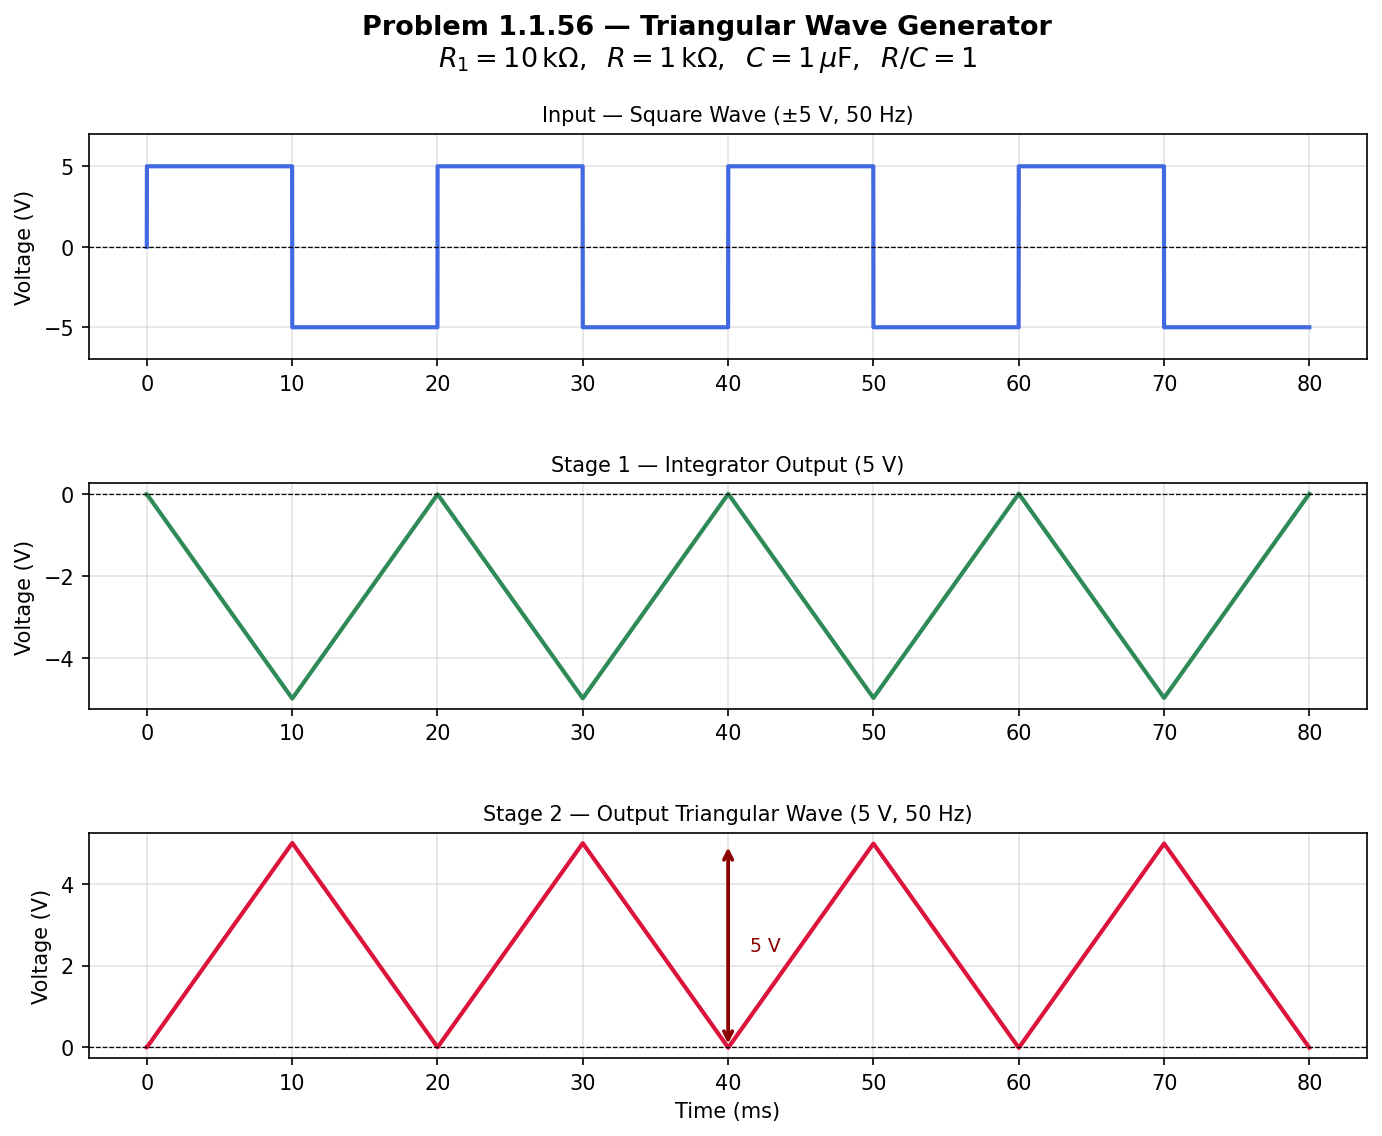
\includegraphics[width=0.7\columnwidth]{figs/waveforms.png} 
  \caption*{Fig : Waveforms}
  \label{Fig1}
\end{figure}


\end{frame}

%-------------------------------------------------------------
\begin{frame}[fragile]{Python Code: Verification}

\lstset{basicstyle=\ttfamily\scriptsize}
\begin{lstlisting}[language=Python]
import numpy as np

# ── Given ─────────────────────────────────────────────────────
Vin_amp = 5.0       # Bipolar square wave amplitude (V), i.e. ±5 V
f       = 50        # Hz
T       = 1.0 / f   # Period = 20 ms
R1      = 10**4      # Integrator input resistor = 10 kΩ  (Ω)
R_in2   = 10**3       # Stage-2 input resistor    =  1 kΩ  (Ω)


# ── Analysis ──────────────────────────────────────────────────
# During the +5V half-cycle, integrator ramps DOWN by delta.
# During the −5V half-cycle, integrator ramps UP by delta.
# Net peak-to-peak at Stage-1 output = delta (one half-swing). 

r_c = (5*2*R1)/(Vin_amp*T) 

r_c = r_c / 10**6

print(f"The value of R/C = {r_c}")
\end{lstlisting}


\end{frame}


%-------------------------------------------------------------
\begin{frame}[fragile]{Python Code: Waveform Simulation}

\begin{lstlisting}[language=Python]
"""
plot_waveforms_1156.py  —  Problem 1.1.56 
Simulate and plot waveforms for the triangular wave generator.
Condition: RC = 1  (R = 1 kΩ, C = 1 µF)
"""
import numpy as np
import matplotlib.pyplot as plt
import matplotlib.gridspec as gridspec

# ── Parameters ────────────────────────────────────────────────
Vin_amp = 5.0    # Bipolar square wave amplitude (V)
f       = 50     # Hz
T       = 1 / f  # Period = 20 ms
R1      = 10e3   # Integrator input resistor (Ω) = 10 kΩ
C       = 1e-6   # Capacitor (F) = 1 µF
R2      = 1e3    # Stage-2 feedback resistor (Ω) = 1 kΩ
R_in2   = 1e3    # Stage-2 input resistor (Ω) = 1 kΩ
gain2   = R2 / R_in2  # = 1

dt = T / 2000
t  = np.arange(0, 4 * T, dt)

# ── Input: bipolar square wave ±5 V ───────────────────────────
Vin = Vin_amp * np.sign(np.sin(2 * np.pi * f * t))

# ── Stage 1: Inverting integrator (Euler) ─────────────────────
Vint = np.zeros(len(t))
for i in range(1, len(t)):
    Vint[i] = Vint[i - 1] - (Vin[i - 1] / (R1 * C)) * dt

\end{lstlisting}


\end{frame}


%-------------------------------------------------------------
\begin{frame}[fragile]{Python Code: Waveform Simulation}

\begin{lstlisting}[language=Python]



# ── Stage 2: Inverting amplifier ──────────────────────────────
Vout = -gain2 * Vint

# ── Measure pp after settling ─────────────────────────────────
mask    = t > T
Vpp_out = Vout[mask].max() - Vout[mask].min()
Vpp_int = Vint[mask].max() - Vint[mask].min()

# ── Plot ──────────────────────────────────────────────────────
fig = plt.figure(figsize=(11, 8))
fig.suptitle(
    "Problem 1.1.56 — Triangular Wave Generator\n"
    r"$R_1 = 10\,\mathrm{k\Omega},\;\;R = 1\,\mathrm{k\Omega},\;\;"
    r"C = 1\,\mu\mathrm{F},\;\;R/C = 1$",
    fontsize=13, fontweight='bold'
)
gs   = gridspec.GridSpec(3, 1, hspace=0.55)
t_ms = t * 1e3

# ── Panel 1: Input ────────────────────────────────────────────
ax1 = fig.add_subplot(gs[0])
ax1.plot(t_ms, Vin, color='royalblue', lw=2.0)
ax1.set_title('Input — Square Wave (±5 V, 50 Hz)', fontsize=10)
ax1.set_ylabel('Voltage (V)')
ax1.set_ylim(-7, 7)
ax1.axhline(0, color='k', lw=0.6, ls='--')
ax1.grid(True, alpha=0.35)

\end{lstlisting}


\end{frame}


%-------------------------------------------------------------
\begin{frame}[fragile]{Python Code: Waveform Simulation}

\begin{lstlisting}[language=Python]


# ── Panel 2: Integrator output ────────────────────────────────
ax2 = fig.add_subplot(gs[1])
ax2.plot(t_ms, Vint, color='seagreen', lw=2.0)
ax2.set_title(
    f'Stage 1 — Integrator Output (5 V)',
    fontsize=10
)
ax2.set_ylabel('Voltage (V)')
ax2.axhline(0, color='k', lw=0.6, ls='--')
ax2.grid(True, alpha=0.35)

# ── Panel 3: Final output ─────────────────────────────────────
ax3 = fig.add_subplot(gs[2])
ax3.plot(t_ms, Vout, color='crimson', lw=2.0)
ax3.set_title(
    f'Stage 2 — Output Triangular Wave (5 V, 50 Hz)',
    fontsize=10
)
ax3.set_ylabel('Voltage (V)')
ax3.set_xlabel('Time (ms)')
ax3.axhline(0, color='k', lw=0.6, ls='--')
ax3.grid(True, alpha=0.35)
# Annotate peak-to-peak arrow
y_max = Vout[mask].max()
y_min = Vout[mask].min()
x_ann = t_ms[mask][len(t_ms[mask])//3]
ax3.annotate('', xy=(x_ann, y_min), xytext=(x_ann, y_max),arrowprops=dict(arrowstyle='<->', color='darkred', lw=1.8))
ax3.text(x_ann + 1.5, (y_max + y_min) / 2,f'5 V', color='darkred', fontsize=9, va='center')
plt.savefig('waveforms.png', dpi=150, bbox_inches='tight')
plt.show()
\end{lstlisting}

\end{frame}

%-------------------------------------------------------------

\end{document}
